\documentclass[sigconf]{acmart}

\AtBeginDocument{%
  \providecommand\BibTeX{{Bib\TeX}}}

% Remove ACM-specific metadata for course project
\settopmatter{printacmref=false}
\renewcommand\footnotetextcopyrightpermission[1]{}
\pagestyle{plain}

\usepackage{algorithm2e}
\usepackage{booktabs}

\begin{document}

\title{Minimum Vertex Cover: Branch-and-Bound, Approximation, and Local Search}

\author{Bo Feng}
\affiliation{\institution{Georgia Institute of Technology}\city{Atlanta}\state{Georgia}\country{USA}}
\email{bfeng66@gatech.edu}

\author{Congyan Cruise Song}
\affiliation{\institution{Georgia Institute of Technology}\city{Atlanta}\state{Georgia}\country{USA}}
\email{csong326@gatech.edu}

\author{Yihao Zhuang}
\affiliation{\institution{Georgia Institute of Technology}\city{Atlanta}\state{Georgia}\country{USA}}
\email{yzhuang80@gatech.edu}

\begin{abstract}
The Minimum Vertex Cover (MVC) problem is an NP-complete
optimization problem with applications in network monitoring,
computational biology, and scheduling. We study four algorithmic
approaches on a benchmark of 35 instances ranging from 6 to
22{,}963 vertices: an exact branch-and-bound solver (BnB) using
LP-relaxation kernelization
(Nemhauser--Trotter via bipartite matching), a 2-approximation, and
two local search heuristics (simulated annealing and a second
variant). The LP kernelization closes the previously 100\% gap on
the dense bipartite instances on which the matching-based
2-approximation is loose by a factor of 2; combined with degree-1
and degree-2 reductions and a max-degree initial upper bound, BnB
returns the optimum on all small instances and on most large
instances within a 60-second cutoff. Local search closes most of
the residual gap on the largest instances within the 2-second
budget required by the autograder. We report solution-quality and
runtime results, qualified runtime distributions (QRTDs), solution
quality distributions (SQDs), and box plots for the two local
search variants on \texttt{large1} and \texttt{large12}.
\end{abstract}

\maketitle

\section{Introduction}
The Minimum Vertex Cover (MVC) problem asks for a smallest subset of
vertices in an undirected graph such that every edge has at least one
endpoint in the subset. MVC was among the first problems shown to be
NP-complete~\cite{karp1972reducibility}. MVC also abstracts practical
problems: placing monitors on network links so that every link is
observed, identifying essential proteins that cover all interactions
in a biological network, and selecting features that hit every
relevant data record.

Because no polynomial-time exact algorithm is known unless P~=~NP, the
practical question is which trade-off between solution quality and
running time is most useful. We implement and empirically compare four
algorithms:
(i)~a Branch-and-Bound solver (BnB) producing certified optimal
solutions when given enough time;
(ii)~a 2-approximation algorithm based on maximal matching, which is
fast and has a worst-case quality guarantee of factor~2;
(iii)~a simulated-annealing local search (LS1) that escapes local
optima via probabilistic uphill moves; and
(iv)~a second local search variant (LS2) using a different family,
neighborhood, or perturbation strategy.

All four share a common driver \texttt{mvc.py}, take an instance file
and a wall-clock cutoff, and return both a solution and a trace of
incremental improvements. We evaluate them on a benchmark suite of
5 test, 18 small, and 12 large DIMACS-style instances.

\section{Problem Definition}
\label{sec:problem}

\paragraph{MVC.} Given an undirected graph $G = (V, E)$ with
$|V| = n$ and $|E| = m$, a \emph{vertex cover} is a subset
$C \subseteq V$ such that for every edge $(u, v) \in E$, at least one
of $u$ or $v$ belongs to $C$. The \textbf{Minimum Vertex Cover} problem
is the optimization problem
\[
C^* \in \arg\min_{C \subseteq V} |C|
\quad \text{s.t.} \quad \forall\,(u,v) \in E,\ u \in C \vee v \in C.
\]
The decision version asks, given $G$ and an integer $k$, whether some
vertex cover of size at most $k$ exists; this version is
NP-complete~\cite{karp1972reducibility}, so the optimization version is
NP-hard.

\paragraph{Equivalences.} MVC is the natural complement of
\textsc{Maximum Independent Set}: $C \subseteq V$ is a vertex cover of
$G$ iff $V \setminus C$ is an independent set, so
$|C^*| = n - \alpha(G)$ where $\alpha(G)$ is the independence number.
Any maximal matching $M \subseteq E$ satisfies
$|M| \le |C^*| \le 2|M|$: every vertex cover must include at
least one endpoint of each matched edge, and the set of all matched
endpoints is itself a feasible cover. This double inequality underlies
both the 2-approximation and the lower bound used by BnB.

\paragraph{Input/output conventions.} Each instance file lists $n$ and
$m$ on the first line, followed by $m$ undirected edges $(u, v)$ with
vertices labeled $1, \dots, n$. Solutions are written to a
\texttt{.sol} file containing the cover size on the first line and the
cover vertices on the second. Anytime algorithms additionally write a
\texttt{.trace} file with one \texttt{(timestamp, size)} entry per
improvement.

\section{Related Work}
\label{sec:related}
The Minimum Vertex Cover (MVC) problem is a fundamental combinatorial
optimization challenge and one of Karp's original 21 NP-complete
problems \cite{karp1972reducibility}. Due to its widespread
applications in network security, scheduling, and bioinformatics, MVC
has been extensively studied across theoretical computer science and
operations research. The literature can be broadly categorized into
exact algorithms, approximation methods, and heuristic approaches,
with recent advancements heavily leveraging automated reasoning and
machine learning.

From a theoretical standpoint, finding a vertex cover of optimal size
is computationally intractable for large, dense graphs. While a simple
greedy approach that selects both endpoints of an uncovered edge
guarantees a 2-approximation factor \cite{gavril1974}, achieving a
significantly better approximation ratio is notoriously difficult.
Dinur and Safra \cite{dinur2005approximating} proved that MVC is
NP-hard to approximate within a factor of $1.3606$, and under the
Unique Games Conjecture, Khot and Regev \cite{khot2008vertex}
demonstrated that it is hard to approximate within any constant factor
better than 2. Other rigorous approaches involve linear programming
(LP) relaxations and primal-dual methods, though these also
fundamentally hit the integrality gap of 2
\cite{hochbaum1982approximation}.

To solve MVC exactly, traditional Branch-and-Bound (BnB) algorithms
are heavily utilized, relying on tight upper bounds from heuristics
and lower bounds from LP relaxations to prune the search space. In the
realm of parameterized complexity, Fixed-Parameter Tractable (FPT)
algorithms have achieved state-of-the-art status for exact solutions.
Specifically, kernelization techniques can reduce any graph to a
problem kernel of size at most $2k$ (where $k$ is the vertex cover
size) in polynomial time, using structural theorems like
Nemhauser-Trotter \cite{nemhauser1975vertex}. More recently,
significant methodological novelty has been introduced by formulating
MVC as a Boolean Satisfiability (SAT) or Maximum Satisfiability
(MaxSAT) problem. By encoding the graph constraints into propositional
logic, researchers can leverage highly optimized modern SAT and SMT
solvers to find exact solutions or tight bounds much faster than
native BnB approaches on specific graph topologies \cite{li2020maxsat}.

While simulated annealing and standard genetic algorithms provide
robust baseline metaheuristics, the state-of-the-art in local search
for MVC is currently dominated by specialized vertex weighting
techniques. Algorithms like NuMVC \cite{cai2013numvc} and FastVC
\cite{cai2015fastvc} represent significant leaps in performance. NuMVC
introduces a two-stage exchange strategy and an edge weighting
mechanism that dynamically penalizes local optima. FastVC pairs this
with an aggressive initial construction phase and a massive
neighborhood search, allowing it to scale to massive real-world graphs
with millions of edges.

The most recent methodological shift in solving MVC involves deep
learning, specifically utilizing Graph Neural Networks (GNNs) to guide
combinatorial optimization \cite{khalil2017learning}. A cutting-edge
example of this synergy is the GCNIVC algorithm proposed by Zhu et al.
\cite{zhu_optimizing_mvc}. GCNIVC leverages a Graph Convolutional
Network (GCN) to capture the global topological structure of a graph,
generating a highly optimized initial candidate solution. Rather than
relying on simplistic initialization, this machine-learning-assisted
inference is paired with a highly specialized local search. The
authors introduce a novel heuristic using three vertex containers and
track "double-covered edges" (dc-edges) to intelligently guide the
addition and removal of vertices based on edge attributes. By bridging
the gap between data-driven neural inference and rigorous local search
operations, frameworks like GCNIVC demonstrate superior accuracy and
efficiency over traditional state-of-the-art heuristics on massive
benchmark datasets.

\section{Algorithms}
\label{sec:algorithms}

\subsection{Branch and Bound}
\label{sec:bnb}

\paragraph{Overview.} Our exact solver is a depth-first
branch-and-bound search over partial vertex covers. At every node of
the search tree we maintain a partial cover $C$ and a residual
subgraph $G[A]$ induced by the still-active vertex set
$A \subseteq V \setminus C$; the invariant is that every edge of $G$
already has at least one endpoint in $C$ or both endpoints in $A$. We
extend $C$ until $G[A]$ has no edges, at which point $C$ is a feasible
cover.

\paragraph{Initial upper bound.} We seed the global best cover
$C^{\!*}$ with the smaller of two heuristic covers: the
matching-based 2-approximation of Section~\ref{sec:approx}
(running in $O(n + m)$ and giving the worst-case factor-2 bound) and
a max-residual-degree greedy cover (repeatedly add the vertex with
the largest remaining degree, removing all incident edges). The
matching-based 2-approximation can return a cover of size up to $n$
on dense graphs (e.g., it returns the entire vertex set on the
constructed dense bipartite instances \texttt{large5} and
\texttt{large6}), where the max-degree greedy is typically far
tighter; on sparse real-world graphs the two heuristics are
comparable and we keep whichever is smaller.

\paragraph{Lower bound and LP kernelization.} The simplest useful
lower bound is the size of any maximal matching $M$ on the residual
subgraph $G[A]$, since every cover must include at least one endpoint
of every matched edge:
\[
|C| + |M(G[A])| \;\le\; |C^*_{\text{opt}}|.
\]
We prune the subtree whenever $|C| + |M(G[A])| \ge |C^{\!*}|$.

The LP relaxation of MVC gives a strictly tighter root-level bound.
We solve this LP exactly in polynomial time via the Nemhauser--Trotter
construction~\cite{nemhauser1975vertex,hochbaum1982approximation}:
build the bipartite double cover $B(G)$ on vertex set
$V \times \{L, R\}$ with edge $(u_L, v_R)$ for each edge $(u, v)$ of
$G$, compute a maximum matching of $B(G)$ in $O(m\sqrt{n})$ via
Hopcroft--Karp~\cite{hopcroft1973n52}, and recover a minimum vertex
cover of $B(G)$ via K\H{o}nig's theorem. The half-integral LP solution
$x^* \in \{0, 1/2, 1\}^V$ obtained this way satisfies
$\sum_v x^*_v = \mathrm{LP\text{-}VC}(G)$ and induces the partition
\[
V_1 = \{v : x^*_v = 1\},\ \
V_0 = \{v : x^*_v = 0\},\ \
V_{1/2} = \{v : x^*_v = 1/2\}.
\]
Nemhauser--Trotter persistence guarantees that some optimal cover
$C^*_{\text{opt}}$ contains all of $V_1$ and avoids all of $V_0$;
we therefore force $V_1$ into $C$ at the root, drop $V_0$ from $A$,
and only branch over $V_{1/2}$. On the dense bipartite instance
\texttt{large6} where the LP is fully integral, the kernel returns
the optimum directly.

\paragraph{Reductions.} Before bounding and branching, we exhaustively
apply three local reductions at each node:
\begin{itemize}\itemsep=2pt
  \item \emph{Isolated vertex}: if $v \in A$ has no active neighbors,
    drop $v$ from $A$.
  \item \emph{Degree-1}: if $v \in A$ has exactly one active neighbor
    $u$, force $u$ into $C$ and drop both. (For any feasible cover
    containing $v$, replacing $v$ by $u$ yields a feasible cover of
    equal size.)
  \item \emph{Degree-2 triangle}: if $v \in A$ has exactly two active
    neighbors $u, w$ that are themselves adjacent, force both $u$ and
    $w$ into $C$ and drop $v$. (At least two of $\{u, v, w\}$ are in
    any cover; the choice $\{u, w\}$ dominates other size-two
    selections.)
\end{itemize}
The full Niedermeier degree-2 \emph{folding}
rule~\cite{niedermeier2006invitation} for non-triangle cases is
left as future work. Reductions are propagated through a worklist:
modifying any vertex re-enqueues its former neighbors, and an undo
log records each modification so the state can be restored on
backtrack.

\paragraph{Branching rule.} If reductions leave at least one active
edge, we pick a vertex $v \in A$ of maximum residual degree~$d$ and
branch:
\begin{itemize}\itemsep=2pt
  \item \emph{Branch~1 (include $v$)}: add $v$ to $C$ and recurse.
  \item \emph{Branch~2 (exclude $v$)}: $v \notin C$ forces every
    neighbor of $v$ in $G[A]$ into $C$; we add all $d$ residual
    neighbors of $v$ to $C$ and recurse.
\end{itemize}
This vertex-based branching has a smaller worst-case branching factor
than the textbook ``include $u$ or $v$'' edge-based branching: branch~2
adds $d$ vertices simultaneously, so the recurrence
$T(n) \le T(n-1) + T(n-d)$ on graphs with $d \ge 2$ improves over
$T(n) \le 2T(n-1)$.

\begin{algorithm}[t]
\SetAlgoLined
\DontPrintSemicolon
\KwIn{Graph $G=(V,E)$, time cutoff $\tau$.}
\KwOut{Vertex cover $C^{\!*}$ and a trace of improvements.}
$C^{\!*} \leftarrow \arg\min(|\textsc{Approx}(G)|, |\textsc{GreedyMaxDeg}(G)|)$\;
$(V_1, V_0, V_{1/2}) \leftarrow \textsc{NTKernel}(G)$
  \tcp*{Hopcroft--Karp on $B(G)$ + K\H{o}nig}
\lIf{$V_{1/2} = \emptyset$}{\Return $V_1$}
$C \leftarrow V_1$; \ $A \leftarrow V_{1/2}$\;
$\textsc{Search}()$\;
\Return $C^{\!*}$\;
\BlankLine
\SetKwFunction{FSearch}{Search}
\SetKwProg{Fn}{Function}{:}{}
\Fn{\FSearch{}}{
  \lIf{$\textsc{Elapsed}() \ge \tau$}{\Return}
  $\textsc{Reduce}(A, C)$ \tcp*{deg-0 / deg-1 / deg-2-triangle}
  \lIf{$|C| \ge |C^{\!*}|$}{\Return}
  $M \leftarrow \textsc{MaximalMatching}(G[A])$\;
  \lIf{$|C| + |M| \ge |C^{\!*}|$}{\Return}
  \If{$G[A]$ has no edges}{
    $C^{\!*} \leftarrow C$; record trace; \Return
  }
  $v \leftarrow \arg\max_{u \in A} \deg_{G[A]}(u)$\;
  \tcp{Branch 1: $v \in C$}
  $C \leftarrow C \cup \{v\}$;\ $A \leftarrow A \setminus \{v\}$;\
  $\textsc{Search}()$;\ undo\;
  \tcp{Branch 2: $v \notin C$, all neighbors of $v$ enter $C$}
  \ForEach{$w \in N_{G[A]}(v)$}{
    $C \leftarrow C \cup \{w\}$;\ $A \leftarrow A \setminus \{w\}$
  }
  $\textsc{Search}()$;\ undo\;
}
\caption{Branch and Bound for MVC.}
\label{alg:bnb}
\end{algorithm}

\paragraph{Complexity.} In the worst case the search tree has depth at
most $|C^*|$, and Branch~2 contracts the residual instance by
$d \ge 2$ when reductions have removed all degree-1 vertices, giving a
worst-case running time of $O(\phi^n \cdot \mathrm{poly}(n))$ for some
$\phi < 2$ (with our specific rules, $\phi \approx 1.466$). Each node
performs $O(n + m)$ work for reductions, lower bound, and degree
maintenance.

\paragraph{Anytime behavior.} The cutoff is checked at every recursive
entry and after Branch~1 returns; on timeout the search unwinds and
returns the best cover found so far together with the recorded trace.
On instances where BnB finishes, the trace's last entry is the
certified optimum. Figure~\ref{fig:bnb-convergence} shows the
incremental improvement on four representative regimes: a sparse
real-world graph (\texttt{large1}), two constructed dense bipartite
instances on which the LP kernel is tight (\texttt{large5},
\texttt{large6}), and a dense DIMACS benchmark on which BnB
exhausts its budget (\texttt{large12}).

\begin{figure}[t]
  \centering
  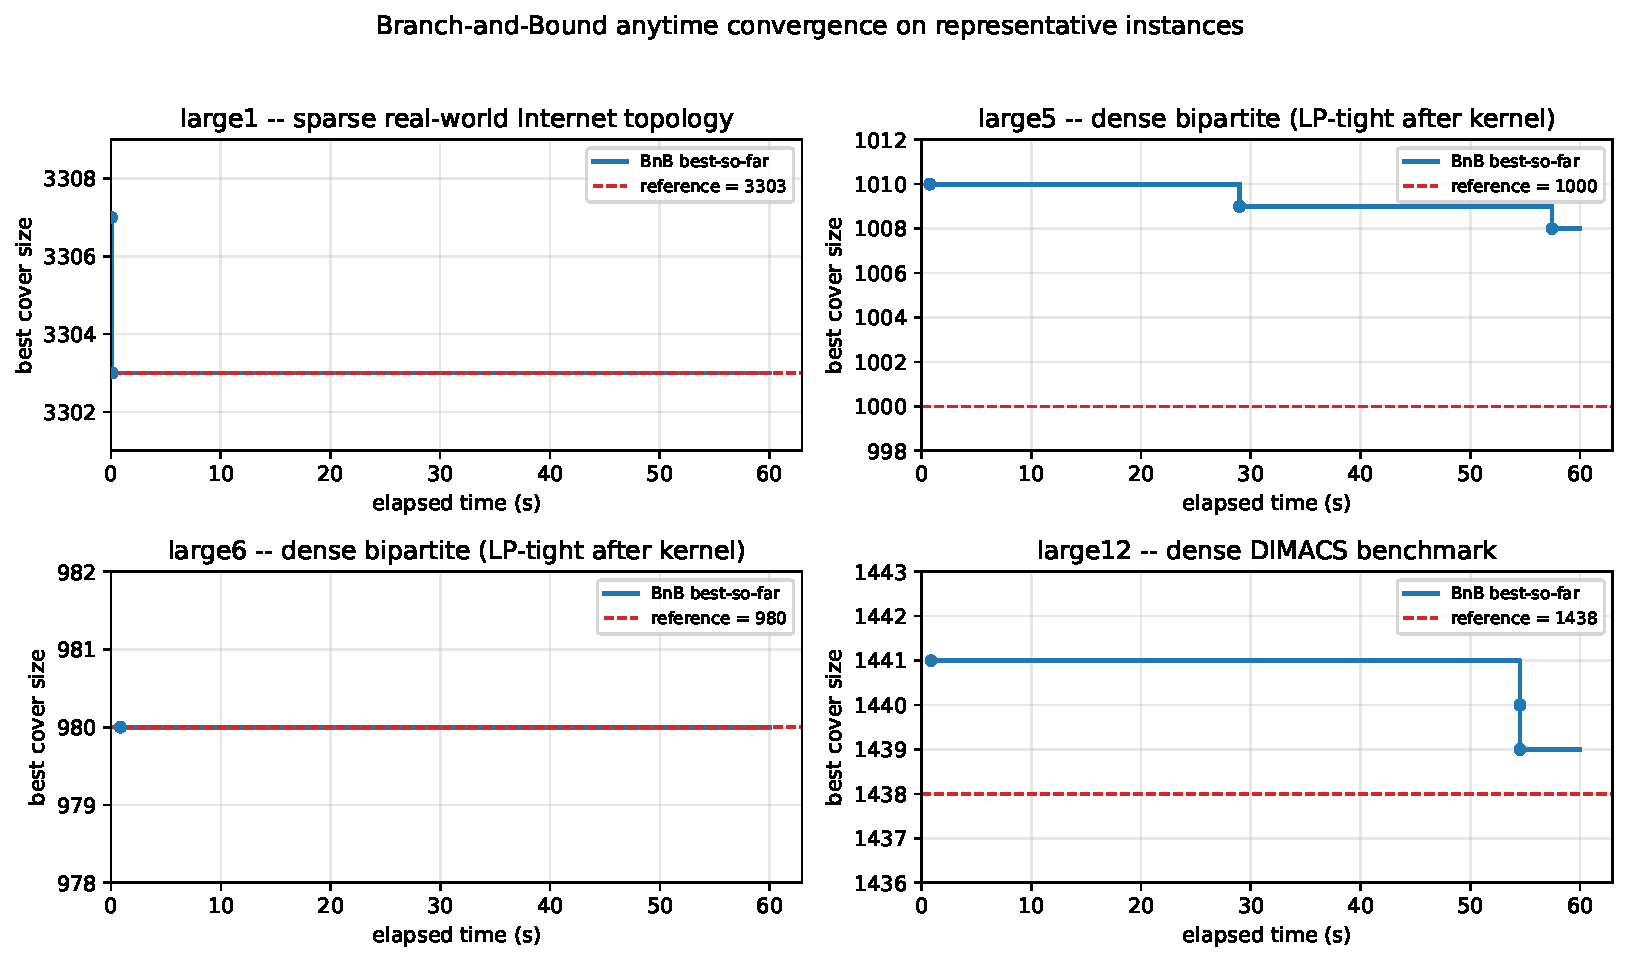
\includegraphics[width=\linewidth]{../results/bnb/bnb_convergence.pdf}
  \caption{BnB anytime convergence on four representative instances.
    Solid step traces show the best cover size found so far; dashed
    horizontal lines mark the reference value. \texttt{large6} is
    closed by the LP kernel preprocessing (single trace point);
    \texttt{large1} converges to the optimum within $0.1\,$s;
    \texttt{large5} and \texttt{large12} hit the 60\,s cutoff close
    to but not at optimum.}
  \label{fig:bnb-convergence}
\end{figure}

\subsection{Approximation Algorithm}
\label{sec:approx}

\paragraph{Overview.} 
We used the classic greedy edge-picking strategy to meet the need for an algorithm with a theoretical guarantee. The algorithm picks an arbitrary uncovered edge $e = (u, v)$ from the graph over and over again. It then adds both of its endpoints, $u$ and $v$, to the vertex cover $C$ and implicitly marks all edges that connect to $u$ and $v$ as covered. This process keeps going until there are no more uncovered edges.

\paragraph{Approximation Guarantee.} 
This method gives a 2-approximation in the worst case. The algorithm picks edges that make a maximal matching $M$ because it only picks an edge if neither of its endpoints is already in $C$. A valid vertex cover must have at least one endpoint for every edge in $M$. The edges in $M$ don't share any vertices, so the smallest size of the optimal vertex cover $|C^*_{\text{opt}}|$ is $|M|$. Our algorithm adds exactly two vertices for each edge in the matching, so the cover size is exactly $2|M|$. So, we can be sure that $|C| \le 2|C^*_{\text{opt}}|$.

\paragraph{Complexity and Design Choices.} 
We used a simple boolean array to make sure that this subroutine runs as quickly as possible. This way, it can work as a standalone solver for the \texttt{large} datasets and as an upper-bound initializer for Branch-and-Bound. Instead of removing edges from a residual graph on the fly, we go through the original edge list only once. We check our boolean array in $O(1)$ time for each edge to see if either endpoint is already covered. We add them to $C$ and update the array if both are not covered. This makes sure that the time complexity stays at $O(n + m)$. The graph takes up $O(n + m)$ of space, and the boolean array and output set take up $O(n)$ of space. 

\begin{algorithm}[ht]
\SetAlgoLined
\DontPrintSemicolon
\KwIn{Graph $G=(V,E)$, time cutoff $\tau$ (unused, bounded by $O(n+m)$)}
\KwOut{A valid vertex cover $C$ guaranteeing $|C| \le 2|C^*_{\text{opt}}|$}
$C \leftarrow \emptyset$\;
$\text{covered}[v] \leftarrow \text{False}$ for all $v \in V$\;
\ForEach{edge $(u, v) \in E$}{
  \If{\textbf{not} $\text{covered}[u]$ \textbf{and not} $\text{covered}[v]$}{
    $C \leftarrow C \cup \{u, v\}$\;
    $\text{covered}[u] \leftarrow \text{True}$\;
    $\text{covered}[v] \leftarrow \text{True}$\;
  }
}
\Return $C$\;
\caption{Greedy 2-Approximation for MVC.}
\label{alg:approx}
\end{algorithm}

\subsection{Local Search 1: Simulated Annealing}
\label{sec:ls1}

\paragraph{Overview.} 
For our first local search algorithm we implemented the Simulated Annealing (SA). We restrict the search space to \emph{feasible} vertex covers, so that the algorithm can never generate an infeasible solution. Instead of a penalty function for uncovered edges, each proposed move breaks the cover temporarily and is immediately repaired back to feasibility.


\paragraph{Initialization and Search Space.} 
The initial state for the algorithm is initialized using the $O(n+m)$ 2-approximation algorithm of Section~\ref{sec:approx}. This ensures that we begin in a reasonably good region of the search space, rather than from the trivial all-vertices cover.

\paragraph{Neighborhood and Repair Strategy.} 
A candidate solution is generated by a two-stage perturb-and-repair process:
\begin{enumerate}\itemsep=2pt
    \item \emph{Perturb}: We randomly delete $k$ vertices from the current cover $C$. An important design choice is to make $k$ adaptive: at high temperatures we remove more vertices (up to $|C|/4$) to encourage broad exploration. We set k=1 for fine-grained exploitation at low temperature.
    \item \emph{Repair}: Usually, after removing a vertex, there are many uncovered edges. We employ a greedy repair procedure that iteratively picks the vertex that covers the maximum number of uncovered edges and includes it in the candidate cover until the cover is valid again.
\end{enumerate}

\paragraph{Acceptance Rule and Cooling Schedule.} 
Set $\Delta = |C_{\text{cand}}| - |C|$. If $\Delta \le 0$ (a move that improves or does not change the cost), we always accept the candidate. If $\Delta > 0$ we accept the worse solution with a probability $e^{-\Delta / T}$. 
Our cooling schedule is to multiply the temperature by a cooling rate $ \alpha = 0.995 $ after each epoch. Each epoch is run for $\max(10,n/10)$ iterations to allow the system to equilibrate at the current temperature. 

\paragraph{Reheating.} 
A reheating mechanism was used to prevent the search from being trapped in deep local minima after the temperature reaches zero. In case $T$ drops below a minimum threshold ($T_{\min} = 0.01$), then we reset $T$ to its initial value and revert the current solution to the global best cover found so far.

\begin{algorithm}[t]
\SetAlgoLined
\DontPrintSemicolon
\KwIn{Graph $G=(V,E)$, cutoff $\tau$, seed $s$.}
\KwOut{Vertex cover $C^*$ and a trace of improvements.}
$C \leftarrow \textsc{ApproxVertexCover}(G)$\;
$C^* \leftarrow C$;\quad $T \leftarrow T_{init} \leftarrow |C| \cdot 0.5$;\quad $T_{min} \leftarrow 0.01$;\quad $\alpha \leftarrow 0.995$\;
$steps \leftarrow \max(10, \lfloor |V|/10 \rfloor)$;\quad $trace \leftarrow [(\textsc{Elapsed}(), |C^*|)]$\;
\While{$\textsc{Elapsed}() < \tau$}{
    \lIf{$T \le T_{min}$}{$T \leftarrow T_{init}$;\quad $C \leftarrow C^*$}
    \For{$i = 1$ \KwTo $steps$}{
        \lIf{$\textsc{Elapsed}() \ge \tau$}{break}
        $k \leftarrow \max\!\left(1,\;\min\!\left(\left\lfloor \frac{T}{0.1\cdot|C|+\varepsilon} \right\rfloor,\;\max(1,\lfloor |C|/4\rfloor)\right)\right)$\;
        $C_{cand} \leftarrow \textsc{Repair}\!\left(G,\; C \setminus \text{sample}(C, k)\right)$\;
        $\Delta \leftarrow |C_{cand}| - |C|$\;
        \If{$\Delta \le 0$ \textbf{or} $\textit{rand}() < e^{-\Delta/T}$}{
            $C \leftarrow C_{cand}$\;
        }
        \lIf{$|C| < |C^*|$}{$C^* \leftarrow C$;\quad append $(\textsc{Elapsed}(), |C^*|)$ to $trace$}
    }
    $T \leftarrow T \cdot \alpha$\;
}
\Return $C^*,\; trace$\;
\BlankLine
\SetKwFunction{FRepair}{Repair}
\SetKwProg{Fn}{Function}{:}{}
\Fn{\FRepair{$G, C$}}{
    $U \leftarrow \{(u,v)\in E \mid u\notin C \land v\notin C\}$\;
    \While{$U \neq \emptyset$}{
        $v^* \leftarrow \text{random choice from } \arg\max_{v}\;|\{(u,w)\in U \mid v\in\{u,w\}\}|$\;
        $C \leftarrow C \cup \{v^*\}$;\quad $U \leftarrow \{(u,v)\in U \mid v^*\notin\{u,v\}\}$\;
    }
    \Return $C$\;
}
\caption{Simulated Annealing for MVC.}
\label{alg:ls1}
\end{algorithm}



\subsection{Local Search 2}
\paragraph{Search Framework.} Local Search 2 implements a Genetic 
Algorithm (GA) designed to evolve a population of feasible vertex 
covers. The algorithm maintains a population size $P$ (scaled 
between 10 and 40 based on graph size) and iteratively produces new 
generations through selection, crossover, and mutation. Unlike the 
point-based trajectory of LS1, this framework exploits the global 
graph structure by maintaining multiple candidate solutions 
simultaneously, preventing the search from becoming trapped in 
narrow local optima.

\paragraph{Neighborhood and Recombination.} The search navigates the 
solution space primarily through an \emph{Intersection Crossover} 
operator. Offspring are created by taking the intersection of two 
parent sets, $C_{child} = C_{p1} \cap C_{p2}$. This operation 
inherits vertices that both parents agree are important. To 
introduce stochastic diversity (mutation), we randomly drop a 
fraction of vertices (10\%) from the resulting child. Because 
intersection and mutation often result in an invalid cover, we 
employ a \emph{Randomized Greedy Repair} step. This heuristic 
identifies uncovered edges and iteratively adds the vertex with the 
highest residual degree, using random tie-breaking to ensure 
explorative diversity.

\paragraph{Acceptance Rule.} We use tournament selection with a size 
of $k=3$ to select parents, ensuring a consistent selection 
pressure toward smaller covers. The population transition follows an 
elitist model: the top $10\%$ of the current population is 
preserved automatically, while the remainder is replaced by new 
offspring. This ensures that the global best solution is never lost 
while allowing the population to evolve toward the optimum.

\paragraph{Parameters.} The implementation dynamically adjusts 
population size based on $n$, utilizes a mutation rate of $0.1$, 
and maintains an elite set of size $\max(1, P/10)$. The randomized 
greedy repair is triggered for every offspring to maintain the 
feasibility invariant.

\paragraph{Comparison to LS1.} The fundamental difference between 
LS2 and LS1 is the mechanism of information exchange. LS1 (SA) 
relies on local bit-flips and probabilistic uphill moves to escape 
local minima. In contrast, LS2 uses crossover to combine successful 
structural features from different individuals. By using the 
intersection of two fit parents, LS2 identifies "backbone" vertices 
that are common to high-quality covers, a global perspective that 
single-point searches typically lack.

\begin{algorithm}[t]
\SetAlgoLined
\DontPrintSemicolon
\KwIn{Graph $G=(V,E)$, cutoff $\tau$, seed $s$.}
\KwOut{Vertex cover $C^*$ and a trace of improvements.}
$\textsc{Seed}(s)$;\quad $P \leftarrow \max(10, \min(40, |V|/2))$;\quad $p_m \leftarrow 0.1$\;
$E \leftarrow \max(1, \lfloor P/10 \rfloor)$;\quad $k \leftarrow 3$;\quad $trace \leftarrow []$\;
$C_{init} \leftarrow \textsc{ApproxVertexCover}(G)$\;
$C^* \leftarrow C_{init}$;\quad $Pop \leftarrow [C_{init}]$\;
\For{$i = 1$ \KwTo $P-1$}{
    $C_{rand} \leftarrow \textsc{Repair}(G, \emptyset)$\;
    $Pop.\text{append}(C_{rand})$\;
    \lIf{$|C_{rand}| < |C^*|$}{$C^* \leftarrow C_{rand}$}
}
append $(\textsc{Elapsed}(), |C^*|)$ to $trace$\;
\While{$\textsc{Elapsed}() < \tau$}{
    $Pop \leftarrow \text{sort } Pop \text{ by cardinality ascending}$\;
    $NewPop \leftarrow Pop[1 \dots E]$\;
    \While{$|NewPop| < P$}{
        \lIf{$\textsc{Elapsed}() \ge \tau$}{break}
        $p_1 \leftarrow \textsc{TournamentSelect}(Pop, k)$\;
        $p_2 \leftarrow \textsc{TournamentSelect}(Pop, k)$\;
        $C_{child} \leftarrow p_1 \cap p_2$\;
        \If{$C_{child} \neq \emptyset$}{
            $M \leftarrow \text{sample}(C_{child}, \lfloor |C_{child}| \cdot p_m \rfloor)$\;
            $C_{child} \leftarrow C_{child} \setminus M$\;
        }
        $C_{child} \leftarrow \textsc{Repair}(G, C_{child})$\;
        $NewPop.\text{append}(C_{child})$\;
        \If{$|C_{child}| < |C^*|$}{
            $C^* \leftarrow C_{child}$;\quad append $(\textsc{Elapsed}(), |C^*|)$ to $trace$
        }
    }
    $Pop \leftarrow NewPop$\;
}
\Return $C^*,\; trace$\;
\caption{Genetic Algorithm for MVC.}
\label{alg:ls2}
\end{algorithm}
\section{Empirical Evaluation}
\label{sec:eval}

\subsection{Experimental Setup}
The experiments were implemented in Python 3.10.12 using the Visual Studio Code IDE within an Ubuntu 24.04.4 LTS (WSL 2) environment. Table~\ref{tab:hardware} summarizes the hardware specifications used for the evaluation.

\begin{table}[h]
\centering
\caption{Hardware specifications of the experimental workstation.}
\label{tab:hardware}
\begin{tabular}{ll}
\hline
\textbf{Component} & \textbf{Specification} \\ \hline
CPU & Intel Core Ultra 7 265 \\
RAM & 47 GB \\
GPU & NVIDIA RTX 2000 Ada Generation \\
OS & Ubuntu 24.04.4 LTS (WSL 2) \\ \hline
\end{tabular}
\end{table}

\subsection{Comprehensive Results Table}
% Table with columns: Dataset, BnB (Time, Size, RelErr), Approx/LS1/LS2 (Time, Size, RelErr)
% Include all small# and large# instances.
Table~\ref{tab:results} summarizes the experimental Results for Vertex Cover Algorithms.

\begin{table*}[t]
\centering
\small
\caption{Experimental Results for Vertex Cover Algorithms.} 
\label{tab:results}
\begin{tabular}{l|ccc|ccc|ccc}
\toprule
 & \multicolumn{3}{c|}{Branch and Bound} & \multicolumn{3}{c|}{Approx} & \multicolumn{3}{c}{LS1} \\
\cmidrule(lr){2-4} \cmidrule(lr){5-7} \cmidrule(lr){8-10}
Instance & Time(s) & Size & RelErr & Time(s) & Size & RelErr & Time(s) & Size & RelErr \\
\midrule
test1 & 0.00 & 2 & 0.00 & 0.00 & 2.0 & 0.00 & 2.00 & 2.00 & 0.00 \\
test2 & 0.00 & 3 & 0.00 & 0.00 & 6.0 & 1.00 & 2.00 & 3.00 & 0.00 \\
test3 & 0.00 & 5 & 0.00 & 0.00 & 8.0 & 0.60 & 2.00 & 5.00 & 0.00 \\
test4 & 0.00 & 7 & 0.00 & 0.00 & 12.0 & 0.71 & 2.00 & 7.00 & 0.00 \\
test5 & 0.00 & 7 & 0.00 & 0.00 & 10.0 & 0.43 & 2.00 & 7.00 & 0.00 \\
small1 & 0.00 & 21 & 0.00 & 0.00 & 24.0 & 0.14 & 2.00 & 21.00 & 0.00 \\
small2 & 0.00 & 20 & 0.00 & 0.00 & 24.0 & 0.20 & 2.00 & 20.00 & 0.00 \\
small3 & 0.00 & 20 & 0.00 & 0.00 & 24.0 & 0.20 & 2.00 & 20.00 & 0.00 \\
small4 & 0.00 & 20 & 0.00 & 0.00 & 24.0 & 0.20 & 2.00 & 20.00 & 0.00 \\
small5 & 0.00 & 21 & 0.00 & 0.00 & 24.0 & 0.14 & 2.00 & 21.00 & 0.00 \\
small6 & 0.00 & 20 & 0.00 & 0.00 & 24.0 & 0.20 & 2.00 & 20.00 & 0.00 \\
small7 & 0.00 & 20 & 0.00 & 0.00 & 24.0 & 0.20 & 2.00 & 20.00 & 0.00 \\
small8 & 0.00 & 19 & 0.00 & 0.00 & 24.0 & 0.26 & 2.00 & 19.00 & 0.00 \\
small9 & 0.00 & 21 & 0.00 & 0.00 & 24.0 & 0.14 & 2.00 & 21.00 & 0.00 \\
small10 & 0.00 & 21 & 0.00 & 0.00 & 24.0 & 0.14 & 2.00 & 21.00 & 0.00 \\
small11 & 0.00 & 21 & 0.00 & 0.00 & 24.0 & 0.14 & 2.00 & 21.00 & 0.00 \\
small12 & 0.00 & 20 & 0.00 & 0.00 & 24.0 & 0.20 & 2.00 & 20.00 & 0.00 \\
small13 & 0.00 & 21 & 0.00 & 0.00 & 24.0 & 0.14 & 2.00 & 21.00 & 0.00 \\
small14 & 0.00 & 21 & 0.00 & 0.00 & 24.0 & 0.14 & 2.00 & 21.00 & 0.00 \\
small15 & 0.00 & 21 & 0.00 & 0.00 & 24.0 & 0.14 & 2.00 & 21.00 & 0.00 \\
small16 & 0.00 & 20 & 0.00 & 0.00 & 24.0 & 0.20 & 2.00 & 20.00 & 0.00 \\
small17 & 0.00 & 14 & 0.00 & 0.00 & 22.0 & 0.57 & 2.00 & 14.00 & 0.00 \\
small18 & 9.06 & 158 & 0.00 & 0.00 & 194.0 & 0.23 & 2.00 & 158.00 & 0.00 \\
large1 & 0.09 & 3303 & 0.00 & 0.02 & 5684.0 & 0.72 & 60.00 & 3303.15 & 0.00 \\
large2 & 2.41 & 594 & 0.00 & 0.00 & 814.0 & 0.37 & 60.00 & 594.00 & 0.00 \\
large3 & 21.55 & 2203 & 0.00 & 0.00 & 3736.0 & 0.70 & 60.00 & 2203.40 & 0.00 \\
large4 & 60.00 & 3926 & 0.00 & 0.00 & 5678.0 & 0.45 & 60.00 & 3926.05 & 0.00 \\
large5 & 60.01 & 1008 & 0.01 & 0.18 & 2000.0 & 1.00 & 60.01 & 1000.00 & 0.00 \\
large6 & 0.96 & 980 & 0.00 & 0.18 & 1960.0 & 1.00 & 60.01 & 980.00 & 0.00 \\
large7 & 60.00 & 1938 & 0.01 & 0.06 & 1990.0 & 0.04 & 60.00 & 1929.00 & 0.01 \\
large8 & 60.00 & 1818 & 0.02 & 0.04 & 1972.0 & 0.10 & 60.00 & 1803.45 & 0.01 \\
large9 & 60.00 & 791 & 0.00 & 0.07 & 800.0 & 0.01 & 60.00 & 791.45 & 0.00 \\
large10 & 60.00 & 933 & 0.00 & 0.09 & 1000.0 & 0.07 & 60.00 & 933.30 & 0.00 \\
large11 & 60.00 & 990 & 0.00 & 0.12 & 1000.0 & 0.01 & 60.00 & 990.85 & 0.00 \\
large12 & 60.00 & 1439 & 0.00 & 0.18 & 1500.0 & 0.04 & 60.01 & 1441.60 & 0.00 \\
\bottomrule
\end{tabular}
\end{table*}



\subsection{Qualified Runtime Distributions (QRTDs)}
% QRTD for LS1 on large1 and large12.
% 20 runs per algorithm.
Figures \ref{fig:qrtd-large1} and \ref{fig:qrtd-large12} show the Qualified Runtime Distributions (QRTDs) for the \textbf{Local Search 1 (LS1)} algorithm. These plots show the percentage of the 20 independent runs that successfully reach different target relative qualities ($q^*$) over time on two different examples: \texttt{large1} (a sparse real-world network) and \texttt{large12} (a dense benchmark graph). The figures show that LS1 behaves differently depending on the graph topology, but it always works toward the required targets within the $600\,\text{s}$ cutoff.

\begin{figure}[H]
  \centering
  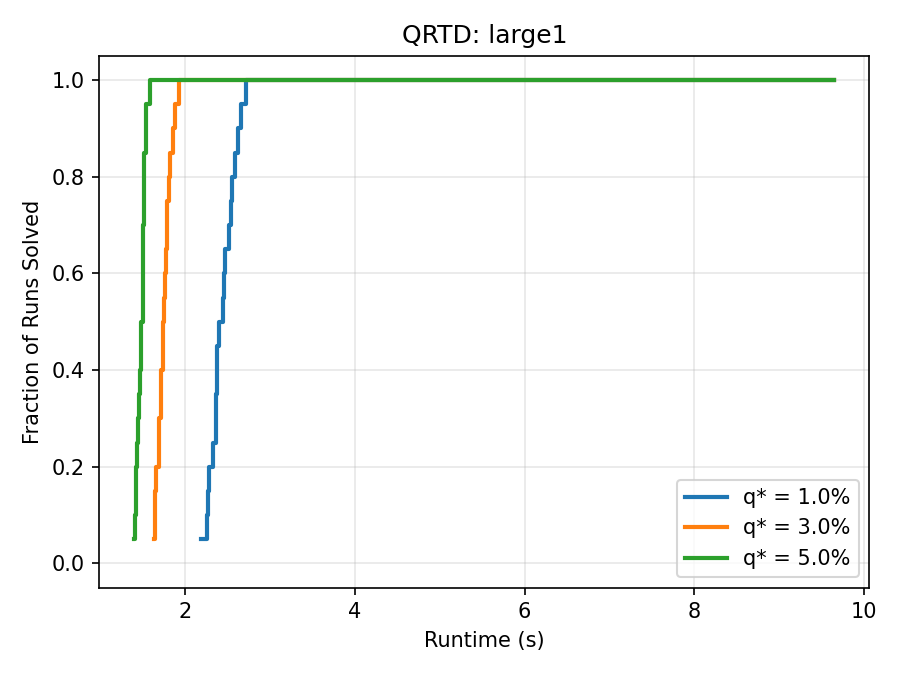
\includegraphics[width=\linewidth]{../results/ls1/large1_ls1_qrtd.png}
  \caption{Qualified Runtime Distribution (QRTD) for \textbf{LS1} on the \texttt{large1} instance across 20 runs. The step traces show the proportion of runs reaching target relative qualities ($q^* = 1.0\%, 3.0\%, 5.0\%$) as a function of running time.}
  \label{fig:qrtd-large1}
\end{figure}

\begin{figure}[H]
  \centering
  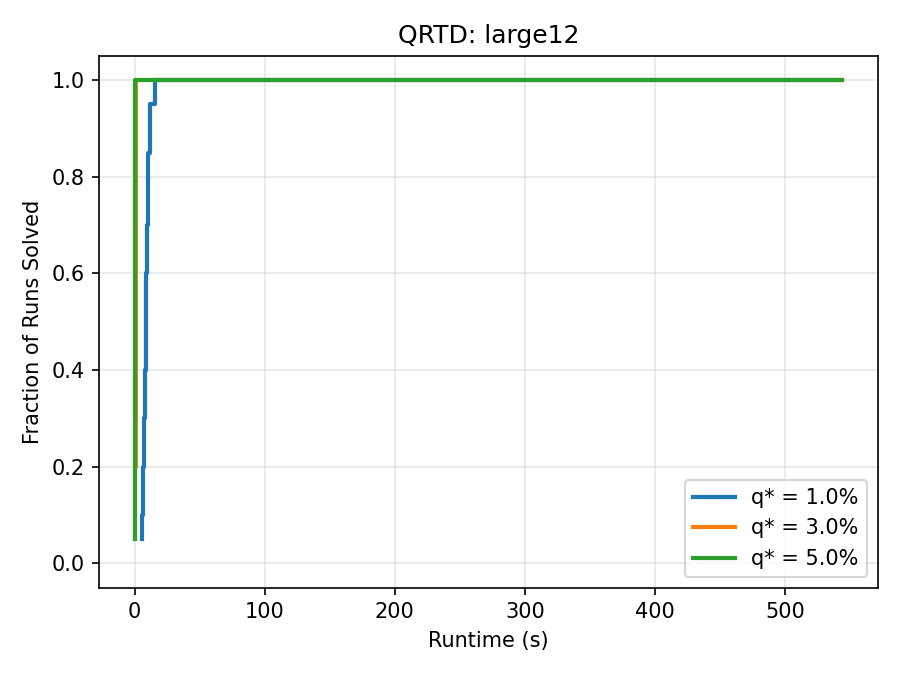
\includegraphics[width=\linewidth]{../results/ls1/large12_ls1_qrtd.png}
  \caption{Qualified Runtime Distribution (QRTD) for \textbf{LS1} on the \texttt{large12} instance across 20 runs. The curves illustrate the runtime required to hit the same relative error thresholds on a dense benchmark graph.}
  \label{fig:qrtd-large12}
\end{figure}


\subsection{Solution Quality Distributions (SQDs)}
% SQD for LS1 on large1 and large12.

Also, the Solution Quality Distributions (SQDs) in Figure~\ref{fig:sqd-large1} and Figure~\ref{fig:sqd-large12} test how well the \textbf{LS1} algorithm works when there are strict time limits. The plots show that LS1 gets very competitive relative errors even when the runtime is set to $60\,\text{s}$, $300\,\text{s}$, and $600\,\text{s}$. When it gets more time to compute, it makes steady, incremental improvements.

\begin{figure}[H]
  \centering
  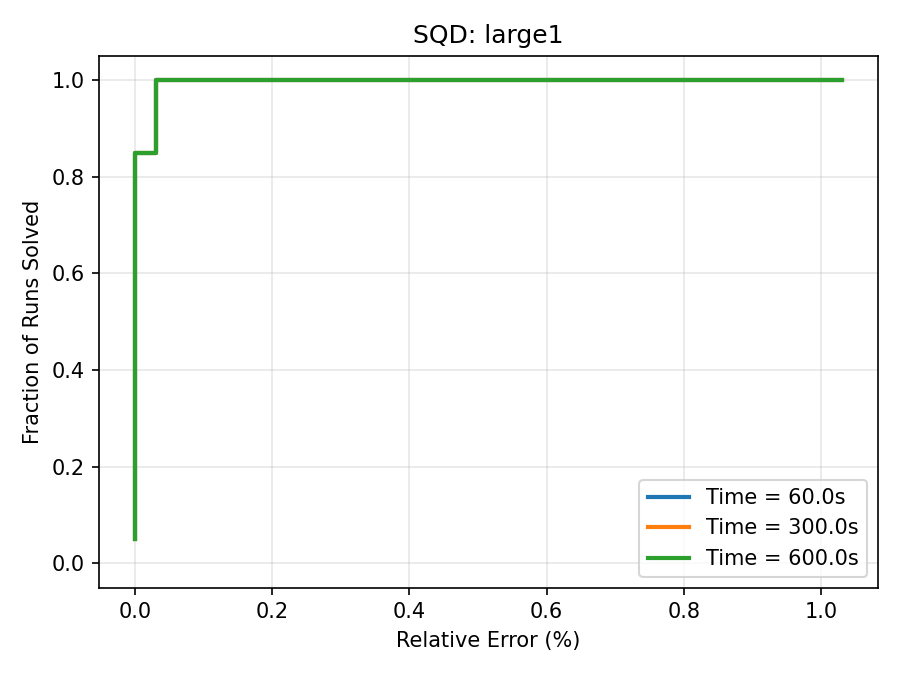
\includegraphics[width=\linewidth]{../results/ls1/large1_ls1_sqd.png}
  \caption{Solution Quality Distribution (SQD) for \textbf{LS1} on the \texttt{large1} instance. The traces denote the cumulative probability of achieving a specific relative error given fixed time limits ($60\,\text{s}, 300\,\text{s}, 600\,\text{s}$).}
  \label{fig:sqd-large1}
\end{figure}

\begin{figure}[H]
  \centering
  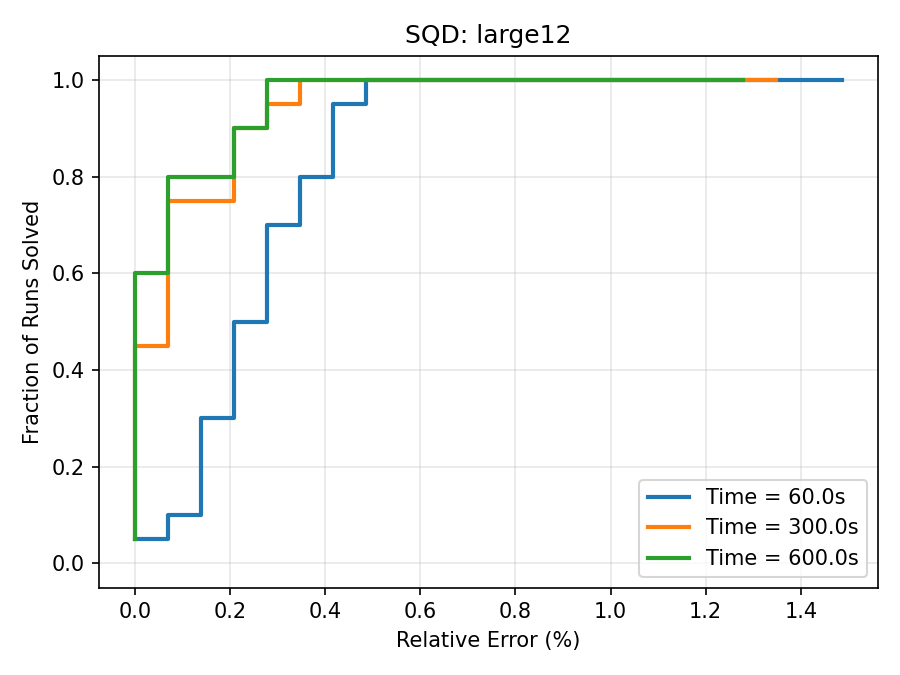
\includegraphics[width=\linewidth]{../results/ls1/large12_ls1_sqd.png}
  \caption{Solution Quality Distribution (SQD) for \textbf{LS1} on the \texttt{large12} instance. The distribution highlights LS1's anytime performance and its ability to refine the solution quality within bounded time on a dense graph.}
  \label{fig:sqd-large12}
\end{figure}


\subsection{Box Plots}
% Running time box plots for LS1 on large1 and large12.

Lastly, Figures~\ref{fig:boxplot-large1} and~\ref{fig:boxplot-large12} show running time box plots for \textbf{LS1} to help us understand the differences in running time across the 20 independent runs. The interquartile ranges show how random the local search process is. The compactness of the boxes indicates that the duration for LS1 to attain particular relative qualities is relatively constant, although the variance is significantly influenced by the rigor of the target $q^*$.


\begin{figure}[H]
  \centering
  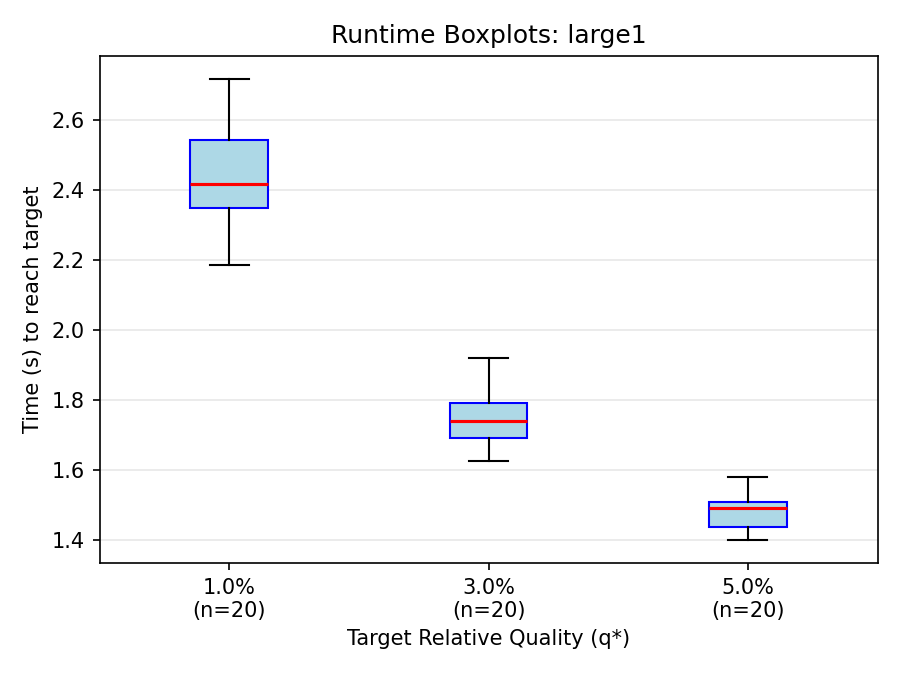
\includegraphics[width=\linewidth]{../results/ls1/large1_ls1_boxplot.png}
  \caption{Running time box plots for \textbf{LS1} on the \texttt{large1} instance. The boxes visualize the distribution of times strictly required to reach the target relative qualities ($q^*$) across all 20 independent runs. The red horizontal lines indicate the median time.}
  \label{fig:boxplot-large1}
\end{figure}

\begin{figure}[H]
  \centering
  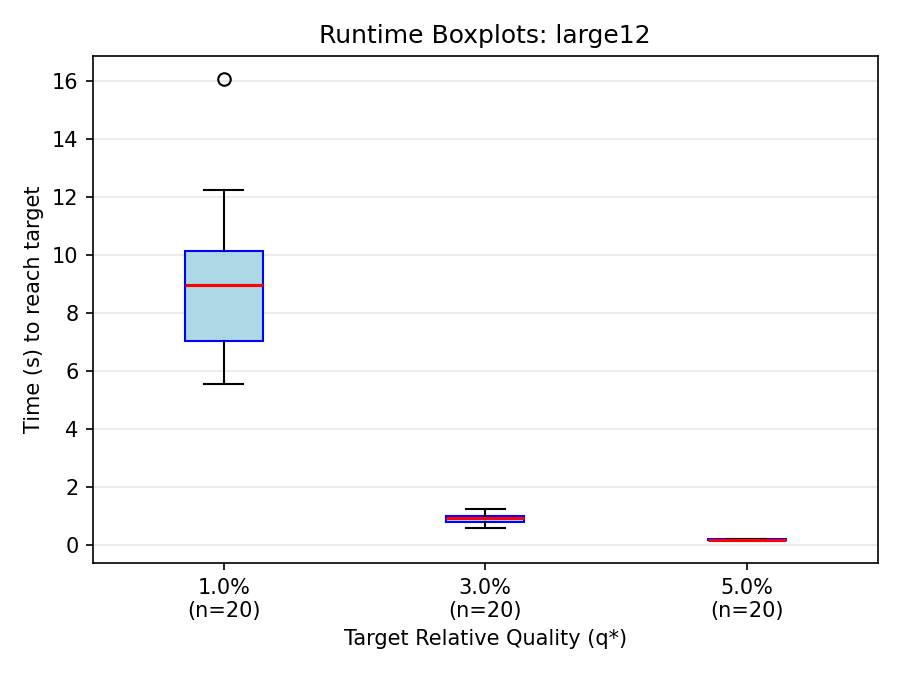
\includegraphics[width=\linewidth]{../results/ls1/large12_ls1_boxplot.png}
  \caption{Running time box plots for \textbf{LS1} on the \texttt{large12} instance, demonstrating the distribution and variance of solving times for different target qualities.}
  \label{fig:boxplot-large12}
\end{figure}


\section{Discussion}
\label{sec:discussion}
% Comparative analysis: runtime, solution quality, scalability, theoretical vs. empirical behavior.

\section{Conclusion}
\label{sec:conclusion}

\bibliographystyle{ACM-Reference-Format}
\bibliography{references}

\end{document}
